\chapter{Methodology}
\label{cha:methodology}

In order to estimate the theoretical bitcoin mining performance, the performance
of the hashing accelerator is measured both when using a DMA for data transfer
and without a DMA. The results are compared to a software implementation of the
algorithm.

In addition to measuring the hashing performance, the power efficiency of the
solution is evaluated, allowing estimating the number of hashes per second per W.

\section{Test Setup}
\label{sec:SHMAC_setup}

To test the accelerator, a 20~tile setup was used on SHMAC. It was decided to include
the following tiles in the design:

\begin{itemize}
    \item 16 CPU tiles with on-tile DMA and SHA256 accelerator
    \item 2 scratchpad tiles
    \item 1 DRAM tile
    \item 1 I/O tile
\end{itemize}

The layout is illustrated in figure \ref{fig:5x4}. The I/O tile is placed to the
left of the first processor in the system, as only the first processor tile is used
for communicating with the host system. This gives the first processor a ``dedicated''
connection to the I/O tile, preventing data that is sent to the host from interferring
with data transfers needed for the hashing benchmark.

\begin{figure}[htb]
    \centering
    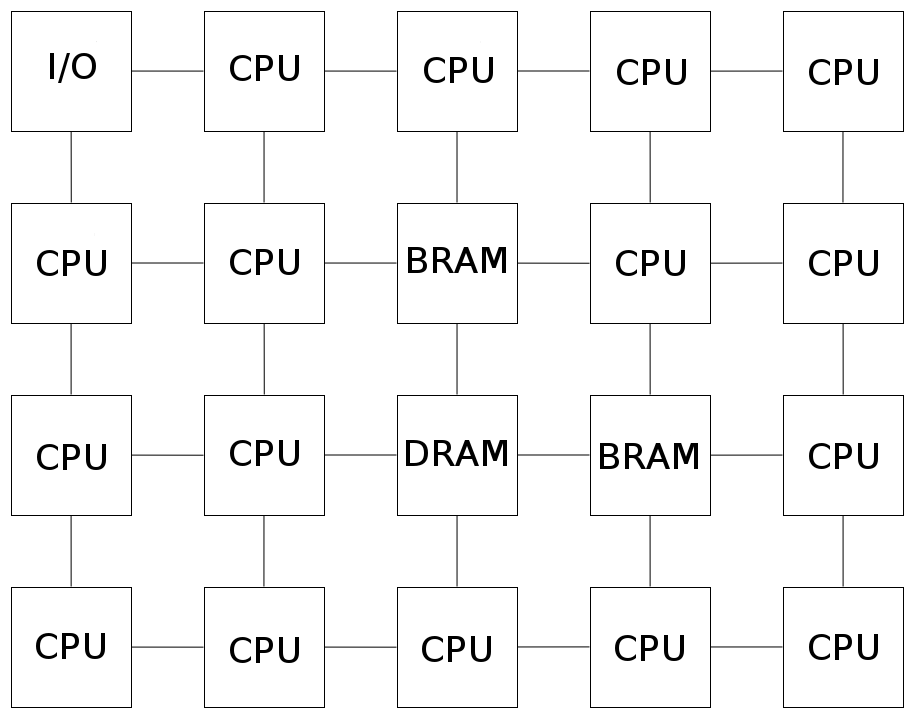
\includegraphics[width=0.5\textwidth]{Figures/Measurements/5x4}
    \caption{Test setup, using BRAM tiles as scratchpad and DRAM as main memory.}
    \label{fig:5x4}
\end{figure}

As testing uncovered a hardware bug in the implementation of the scratchpad tiles,
discussed in section \ref{sec:init-hw-results}, a second design had to be created
in order to measure the scaling of the performance when using accelerators.

The second design places all processor tiles in a single row. This causes all traffic
to the memory tiles, placed on the row below, to come from above, which bypasses the
scratchpad bug previously mentioned.

The design contains 12 CPU tiles and is illustrated in figure \ref{fig:13x2}.

\begin{figure}[htb]
    \centering
    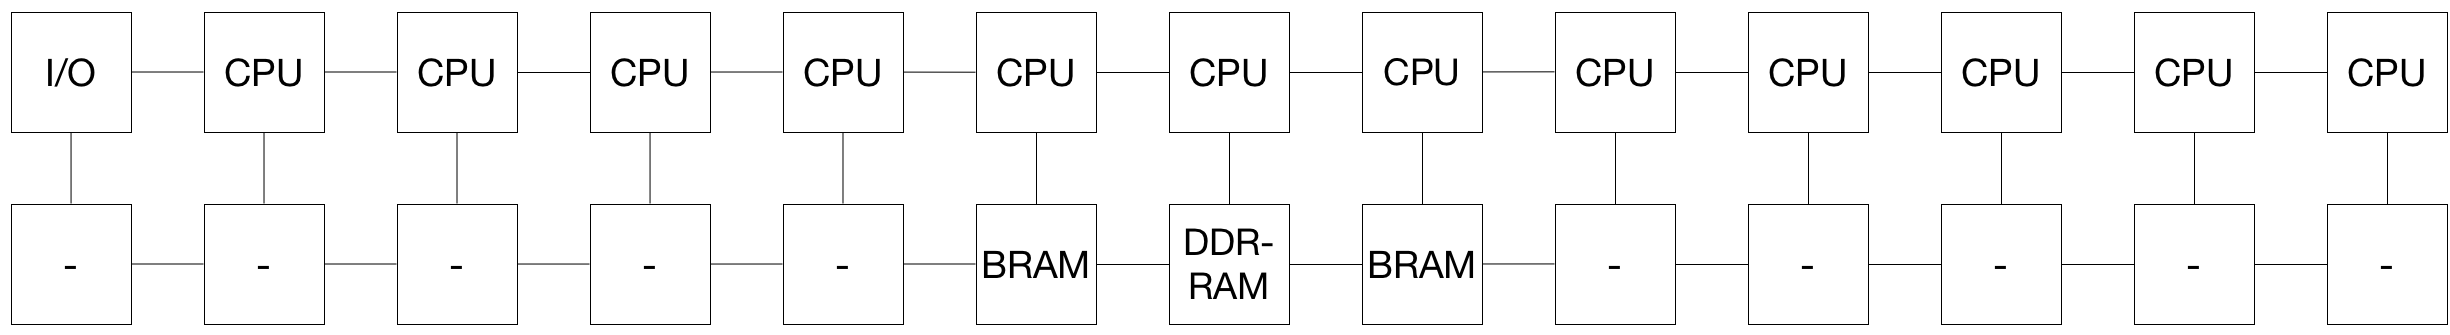
\includegraphics[width=1.0\textwidth]{Figures/Measurements/13x2}
    \caption{Second test setup, with BRAM and DRAM tiles on second row, and all CPUs on the first row.}
    \label{fig:13x2}
\end{figure}

The test designs were synthesized using Xilinx' Vivado software suite, version 2013.4, and
uploaded to a Versatile Express machine\todo{Technical details here}.

\section{Measuring the Performance}

Measuring the performance is done by repeatedly double-hashing a block of data, recording the
number of hashes achieved per second per core. By turning on one core at a time, it
is possible to see how the performance scales as more cores are added. Recording
the number of hashes per second per core makes it possible to see how the performance
of each core is affected by the traffic on the network-on-chip generated by the other
cores in the network.

Using the setup described in section \ref{sec:SHMAC_setup}, tests where run using the
following method:

\begin{itemize}
    \item Hashing using software only, not using the SHA256 hashing module or DMA module.
    All work is done by the on-tile processor.
    \item Hashing using only the hashing accelerator.
    The processor controls and copies data to and from the hashing module.
    \item Hashing using the hashing accelerator and DMA.
    The processor controls each module, but the DMA handles data transfer.
\end{itemize}

Interrupts are used by the hashing module to signal when it is finished working. However,
%the DMA does not support interrupts and has to be polled while copying data to and from
the software does not support interrupt from DMA, and it has to be polled while copying data to and from
the module, which may have a minor influence on the results.

The benchmark software was compiled using the GCC compiler, version 4.8.2, compiled for
the arm-none-eabi target triplet. To generate a binary file for the SHMAC, utilities
from GNU Binutils version 2.24, also compiled for the arm-none-eabi target triplet,
were used.

\section{Measuring Power Usage}
\label{sec:power-measure}

Power usage for the application is determined by measuring the wall-power of the box
that SHMAC is running on both when idle and when running the test applications. The
power usage of the application is then determined using the following formula, where
$P$ is the power in watts:

\[P_{application} = P_{running} - P_{idle}\]

Using the result of the power measurement, the energy efficiency can be obtained as
the number of hashes per second per watt.

To obtain the power usage of SHMAC, a Yokogawa WT210 power meter was used to measure
the power drawn by the Versatile Express box from the power socket in the wall while
idle and when running the bitcoin application. This method provides some uncertainty
in the result of the measurements, as the Versatile Express also runs a Linux host
system, it was not possible to obtain power measurements directly from the FPGA running
SHMAC. % Cannot find a source for the power measurement instrumentation that is in-the-works.
\todo{Remember to underline this uncertainty in the discussion/evaluation part, since}


% FOLLOWING POST-MEETING:
%
%Optional: Write the expected max performance if we can calculate them?
%
%\section{Known hazards with SHMAC and test setup}
%List up potential problems that SHMAC may give us, due to the known bugs in the system (cache coherency issues with DMA, the infamous cache bug.
%
%Also include the uncertainty with testing of wall-power, and the lack of on-chip power measurement.
%
%\section{Tools and software used for this project}
%- Modelsim?
%
%\subsection{Other properties of Vexpress}
%FIND: DDR MEMORY LATENCY AND THROUGHPUT IF POSSIBLE.
%Throughput according to Asbjørn: 128-bit word per cycle.
%Clock is a 50MHz.

